\documentclass[12pt,a4paper]{article}

% Language setting
\usepackage[british]{babel}

% Set page size and margins
\usepackage[a4paper,top=2cm,bottom=2cm,left=2.5cm,right=2.5cm,marginparwidth=1.75cm]{geometry}

%----------- APA style references & citations (starting) ---
% Useful packages
%\usepackage[natbibapa]{apacite} % APA-style citations.

\usepackage[style=apa, backend=biber]{biblatex} % APA 7th edition style citations using biblatex
\addbibresource{references.bib} % Your .bib file

% Formatting DOI in APA-7 style
%\renewcommand{\doiprefix}{https://doi.org/}

% Add additional APA 7th edition requirements
\DeclareLanguageMapping{british}{british-apa} % Set language mapping
\DeclareFieldFormat[article]{volume}{\apanum{#1}} % Format volume number

% Modify 'and' to '&' in the bibliography
\renewcommand*{\finalnamedelim}{%
  \ifnumgreater{\value{liststop}}{2}{\finalandcomma}{}%
  \addspace\&\space}
  
%----------- APA style references & citations (ending) ---


\usepackage{amsmath}
\usepackage{graphicx}
\usepackage[colorlinks=true, allcolors=blue]{hyperref}
\usepackage{hyperref}
\usepackage[title]{appendix}
\usepackage{mathrsfs}
\usepackage{amsfonts}
\usepackage{booktabs} % For \toprule, \midrule, \botrule
\usepackage{caption}  % For \caption
\usepackage{threeparttable} % For table footnotes
\usepackage{algorithm}
\usepackage{algorithmicx}
\usepackage{algpseudocode}
\usepackage{listings}
\usepackage{enumitem}
\usepackage{chngcntr}
\usepackage{booktabs}
\usepackage{lipsum}
\usepackage{subcaption}
\usepackage{authblk}
\usepackage[T1]{fontenc}    % Font encoding
\usepackage{csquotes}       % Include csquotes
\usepackage{diagbox}

%Image-related packages
\usepackage{graphicx}
\usepackage{subcaption}
\usepackage[export]{adjustbox}
\usepackage{wrapfig}

% Customize line spacing
\usepackage{setspace}
\onehalfspacing % 1.5 line spacing

% Redefine section and subsection numbering format
\usepackage{titlesec}
\titleformat{\section} % Redefine section numbering format
  {\normalfont\Large\bfseries}{\thesection.}{1em}{}

% Define a new command for the fourth-level title.
\newcommand{\subsubsubsection}[1]{%
  \vspace{\baselineskip}% Add some space
  \noindent\textbf{#1\\}\quad% Adjust formatting as needed
}
% Change the position of the table caption above the table
\usepackage{float}   % for customizing caption position
\usepackage{caption} % for customizing caption format
\captionsetup[table]{position=top} % caption position for tables

% Define the unnumbered list
\makeatletter
\newenvironment{unlist}{%
  \begin{list}{}{%
    \setlength{\labelwidth}{0pt}%
    \setlength{\labelsep}{0pt}%
    \setlength{\leftmargin}{2em}%
    \setlength{\itemindent}{-2em}%
    \setlength{\topsep}{\medskipamount}%
    \setlength{\itemsep}{3pt}%
  }%
}{%
  \end{list}%
}
\makeatother

% Suppress the warning about \@parboxrestore
\pdfsuppresswarningpagegroup=1


%-------------------------------------------
% Paper Head
%-------------------------------------------
\begin{figure}
    \vspace{-2.5\baselineskip}
    \hspace{12\baselineskip}
    
\includegraphics[width=0.2\textwidth]{figures/Shiraz_University_logo.png}
    \vspace{-3\baselineskip}
\end{figure}

\title{\textbf{Cooley-Tukey FFT Algorithm}}
\author[1]{Seyed Mahdi Mahdavi Mortazavi}
\affil[1]{\small \textit{Department of Electrical and Computer Engineering, Shiraz University}}

\date{}  % Remove date
\begin{document}
\maketitle

\begin{abstract}
The Cooley-Tukey algorithm is a widely used method for efficiently computing the Fast Fourier Transform, a crucial tool in signal processing and data analysis. This review article, explores the development and workings of the Cooley-Tukey algorithm, providing a detailed explanation of its recursive divide-and-conquer approach that enable it to reduce the computation time of the FFT. Additionally, a practical test is provided to understand the effects of this optimization.
\end{abstract}

\textbf{Keywords}: DFT, FFT, Cooley-Tukey Algorithm, Radix-2 DIT, Divide-And-Conquer.  

%-------------------------------------------
% Paper Body
%-------------------------------------------
%--- Section ---%
\section{Introduction}
\hspace{0.5cm} Often in Digital Signal Processing applications, it is necessary to estimate the signal spectrum or vice versa, knowing the signal spectrum calculate the signal itself. For this purpose, digital technology uses the Discrete Fourier Transform (DFT) [\href{https://www.dsp-weimich.com/digital-signal-processing/fast-fourier-transform-fft-and-their-c-realizations-using-the-octave-gnu-tool/}{1}].

DFT operation is useful in many fields, but computing it directly from the definition is often too slow to be practical. A Fast Fourier Transform (FFT) algorithm, rapidly computes such transformations by factorizing the DFT matrix into a product of sparse factors, many of which are zero [\href{https://en.wikipedia.org/wiki/Fast_Fourier_transform#cite_note-Loan_1992-2}{2}].

By far, the most commonly used FFT is the Cooley–Tukey algorithm. This is a divide-and-conquer algorithm that recursively breaks down a DFT of any composite size $n=n_{1}n_{2}$ into many smaller DFTs of sizes $n_{1}$ and $n_{2}$, along with $O(n)$ multiplications [\href{https://en.wikipedia.org/wiki/Fast_Fourier_transform#cite_note-Gentleman_Sande_1966-18}{3}]. As a result, it reduces the complexity of computing the DFT from $O(n^2)$, which arises if one simply applies the definition of DFT, to $O(nlogn)$, where $n$ is the data size. [\href{https://en.wikipedia.org/wiki/Fast_Fourier_transform}{4}].

%--- Section ---%
\section{Cooley-Tukey Algorithm}\label{sec2}
\hspace{0.5cm} The Cooley–Tukey algorithm, named after J. W. Cooley and John Tukey, is the most common FFT algorithm. It transforms the DFT of an arbitrary composite size $N=N_{1}N_{2}$ in terms of N1 smaller DFTs of sizes $N2$, recursively, to reduce the computation time to $O(N log N)$ for highly composite $N$.

\subsection{The radix-2 DIT case}
\hspace{0.5cm} A radix-2 decimation-in-time (DIT) FFT is the simplest and most common form of the Cooley–Tukey algorithm, although highly optimized Cooley–Tukey implementations typically use other forms of the algorithm. Radix-2 DIT divides a DFT of size N into two interleaved DFTs of size $N/2$ with each recursive stage. The DFT is defined by the formula:\\
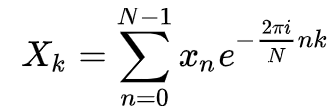
\includegraphics[width=0.3\textwidth]{figures/DFT formula.png}\\
Where $k$ is an integer ranging from $0$ to $N-1$.

Radix-2 DIT computes the DFTs of the even-indexed inputs $(x_{2m}=x_{0},x_{2},\ldots ,x_{N-2})$ and of the odd-indexed inputs $(x_{2m+1}=x_{1},x_{3},\ldots ,x_{N-1})$, and then combines those two results to produce the DFT of the whole sequence. This idea can then be performed recursively to reduce the overall runtime to $O(NlogN)$. This simplified form assumes that $N$ is a power of two. 

The radix-2 DIT algorithm rearranges the DFT of the function $x_{n}$ into two parts: a sum over the even-numbered indices $n=2m$ and a sum over the odd-numbered indices $n=2m+1$:\\
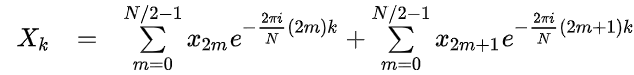
\includegraphics[width=0.85\textwidth]{figures/DFT simplification 1.png}

One can factor a common multiplier $e^{-{\frac {2\pi i}{N}}k}$ out of the second sum, as shown in the equation below. It is then clear that the two sums are the DFT of the even-indexed part $x_{2m}$ and the DFT of odd-indexed part $x_{2m+1}$ of the function $x_{n}$. Denoting the DFT of the Even-indexed inputs $x_{2m}$ by $E_{k}$ and for the Odd-indexed inputs $x_{2m+1}$ by $O_{k}$ and we obtain:\\
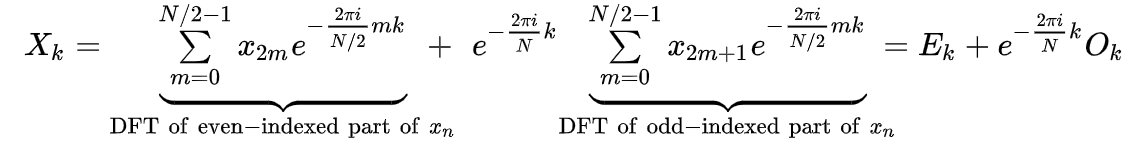
\includegraphics[width=1\textwidth]{figures/DFT simplification 2.png}
Using periodicity of the complex exponential, $X_{k+{\frac {N}{2}}}$ is also obtained from $E_{k}$ and $O_{k}$:\\
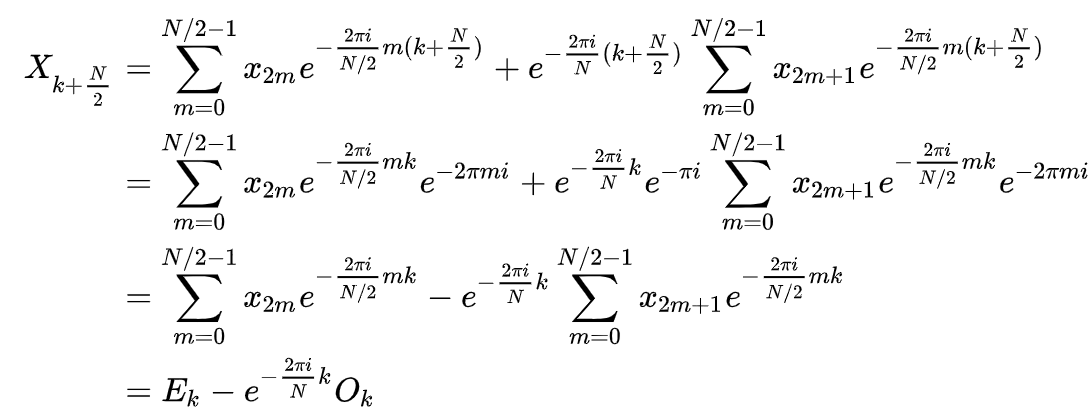
\includegraphics[width=1\linewidth]{figures/DFT simplification 3.png}
We can rewrite $X_{k}$ and $X_{k+{\frac {N}{2}}}$ as [\href{https://en.wikipedia.org/wiki/Cooley%E2%80%93Tukey_FFT_algorithm}{5}]:\\
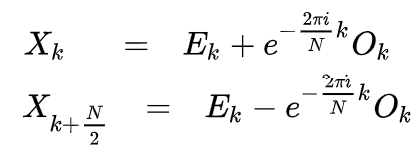
\includegraphics[width=0.45\linewidth]{figures/Final Cooley-Tukey FFT formula.png}

\subsection{Comparison of calculation speed}\label{subsec1}
\hspace{0.5cm} Table 1 presents a comparison of computational speeds between the FFT using the Cooley-Tukey algorithm and the DFT. This comparison highlights the superior computational efficiency of FFT over DFT.
\begin{table}[!ht]
\caption{Comparing the speed of FFT and DFT calculations (approximate) [\href{https://github.com/theMHD-120/fft}{6}]\label{tab1}}
\begin{threeparttable}
\begin{tabular*}{\columnwidth}{@{\extracolsep\fill}llll@{\extracolsep\fill}}
\toprule
Input size & $N = 2^{10}$ & $N = 2^{15}$ & $N = 2^{20}$\\
\midrule
DFT & 1.553 seconds & 26 minutes & 5 hours \\
FFT & 0.055 seconds & 1.564 seconds & 52.218 seconds \\
\bottomrule
\end{tabular*}
\end{threeparttable}
\end{table}

%--- Section ---%
\section{Conclusion}\label{sec3}
\hspace{0.5cm} Expressing the DFT of length $N$ recursively in terms of two DFTs of size $N/2$, is the core of the radix-2 DIT Fast Fourier Transform. The algorithm gains its speed by re-using the results of intermediate computations to compute multiple DFT outputs. Note that final outputs are obtained by a plus and minus combination of $E_{k}$ and $O_{k}\exp(-2\pi ik/N)$, which is simply a size-2 DFT (sometimes called a butterfly in this context); when this is generalized to larger radices, the size-2 DFT is replaced by a larger DFT. This process is an example of the general technique of divide-and-conquer algorithms [\href{https://en.wikipedia.org/wiki/Cooley%E2%80%93Tukey_FFT_algorithm}{5}].

\begin{thebibliography}{9}
\bibitem{texbook}
https://www.dsp-weimich.com/digital-signal-processing/fast-fourier-transform-fft-and-their-c-realizations-using-the-octave-gnu-tool/

\bibitem{texbook}
Van Loan, Charles (1992). Computational Frameworks for the Fast Fourier Transform.

\bibitem{texbook}
Gentleman, W. Morven; Sande, G. (1966). "Fast Fourier transforms—for fun and profit".

\bibitem{texbook}
https://en.wikipedia.org/wiki/Fast\_Fourier\_transform

\bibitem{texbook}
https://en.wikipedia.org/wiki/Cooley-Tukey\_FFT\_algorithm

\bibitem{texbook}
https://github.com/theMHD-120/fft
\end{thebibliography}

\end{document}